\documentclass{article}
\usepackage{comment}
\usepackage{graphicx}
\usepackage{amsmath}
\usepackage{amssymb}
\usepackage{caption}
\usepackage{subcaption}
\usepackage{systeme}
\usepackage{bm}
   \usepackage{hyperref}
    \hypersetup{
    colorlinks=true,
    linkcolor=black,
    filecolor=black,      
    urlcolor=black,
}

%\setcounter{section}{-1}
\title{Double Pendulum: Deterministic but not so Predictable}
\author{H. M. Chu  \\
	Physics Simulation Lab  \\
		%\and 
	%The Other Dude \\
	%His Company / University \\
	}

\date{\today}
% Hint: \title{what ever}, \author{who care} and \date{when ever} could stand 
% before or after the \begin{document} command 
% BUT the \maketitle command MUST come AFTER the \begin{document} command! 
\begin{document}

\maketitle


\begin{abstract}
Though often employed as a way to reduce the complexity of systems of nonlinear equations of double pendulum, nondimensionalization may look like an intuitive, albeit random guess. Nondimensionalization is a powerful technique not only utilized to simplify equations but also to show the interdependent relationship among variables. Justification of nondimensionalization is introduced, although explitcit proof is omitted. Due to its simple configuration, analysis of the dynamics of double pendulum is often used as an entry point to gain insight into the nature of chaos. For an idealized, non-dissipative deterministic dynamical system of double pendulum, the largest Lyapunov exponent (LLE) is one of the best indicators of chaos. In this article, the theoretical basis for the calculation of the characterstic LLE for the double pendulum is presented. The stability of the four fixed points of the double pendulum is also examined. 

\end{abstract}

\section{Introduction}

As the name suggests, a double pendulum is made of two pendula, with one attached to the other, and both are suspended from massless, frictionless wires. For simplicity, our system is assumed to be ideal, i.e., there neither is damping nor external forces so the system could go onto infinity.

Here, our double pendulum has two masses $m_1$ and $m_2$, lengths $l_1$ and $l_2$, respectively. The angles the lengths make with the vertical will be $\theta_1$ and $\theta_2$. Moreover, the gravity is $g$. 

% insert image of pend here

\begin{figure}[h]
\centering
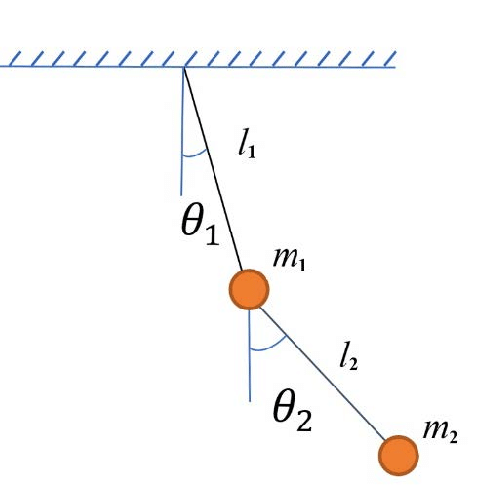
\includegraphics[width=0.5\linewidth]{pend.png}
\caption{Idealized double pendulum}
\end{figure}

To study the dynamics of the system of double pendulum, Lagrangian formalism is chosen. In Cartesian coordinates, the positions of the each of the pendula is given by

% insert positions
\begin{align}
\centering
x_1 &= l_1 \sin\theta_1 \\
y_1 &= -l_1\cos\theta_1 \\
x_2 &= l_1\sin\theta_1 + l_2\sin\theta_2\\
y_2 &= -l_1\cos\theta_1 - l_2 \cos\theta_2
\end{align}

with $(x_1, y_1)$, $(x_2, y_2)$ being the coordinates of mass 1 and mass 2, respectively.

Since the gravitational acceleration $g$ is pointed downward, the potential energy of the system is then

% insert potential
\begin{align}
\centering
V &= m_1gy_1 + m_2gy_2 \\
	&= -(m_1 + m_2)gl_1\cos\theta_1 - m_2gl_2\cos\theta_2
\end{align}

and the kinetic energy is given by

% insert kinetic

\begin{equation}
\centering
\begin{split}
T &= \frac{1}{2}m_1v_1^2+\frac{1}{2}v_2^2 \\
&= \frac{1}{2}l_1^2\dot{\theta}_1^2 + \frac{1}{2}m_2[l_1^2\dot{\theta}_1^2 + l_2^2\dot{\theta}_2^2 + 2l_1l_2\dot{\theta}_1\dot{\theta}_2\cos(\theta_1 - \theta_2)]
\end{split}
\end{equation}

The Lagrangian is then
% insert Lagrangian

\begin{equation}
\begin{split}
L &= T - V \\
&= \frac{1}{2}(m_1+m_2)l_1^2\dot{\theta}_1^2 + \frac{1}{2}m_2l_2^2\dot{\theta}_2^2 + m_2l_1l_2\dot{\theta}_1\dot{\theta}_2\cos(\theta_1 - \theta_2)
\end{split}
\end{equation}

Substitute the Lagrangian into the Euler-Langrange equation

% insert euler-lagrange
\begin{equation}
\frac{d}{dt} \left(\frac{\partial}{\partial \dot{\theta}_n} \right) - \frac{\partial L}{\partial \theta n} = 0, \, n \in {1, 2}
\end{equation}
we obtain the final equations of motion

\begin{equation} \label{eq:10}
(m_1+m_2)l_1^2 \ddot \theta_1 + m_2l_1l_2\ddot \theta_2 \cos(\theta_1 - \theta_2) + m_2l_1l_2\dot \theta_1 \dot \theta_2 \sin(\theta_1 - \theta_2) + gl_1 \sin\theta_1(m_1 + m_2) = 0
\end{equation}

\begin{equation} \label{eq:11}
m_2l_2^2\ddot \theta_2 + m_2l_1\ddot \theta_1\cos(\theta_1 - \theta_2) - m_2l_1l_2\dot \theta_1^2 sin(\theta_1 - \theta_2) + gm_2l_2sin\theta_2 = 0
\end{equation}

% insert equation of motion

\section{Nondimensionalization}

The system of equations 3 suggests nonlinearity. As a result, it's not possible to find a closed form solution for the equation. However, when the angle displacements are small, equations 3 become linear and an analytic solution can be obtained. Generally, numerical methods are employed to investigate the dynamics of double pendulum. 

In order to simplify equations 3, we can employ nondimensionalization. The rationale for nondimensionlization is provided by Buckingham $\pi$ theorem, which states, \textit{"If there are n variables in a problem and these variables contain m primary dimensions (for example m, l, t) the equation relating all the variables will have (n-m) dimensionless groups.} Nondimensionalization also exemplifies the relationships among parameters. We will see why after nondimensionalizing equations of the double pendulum (\ref{eq:10}) and (\ref{eq:11}).

Suppose if we have this physically meaningful equation:


\begin{equation}
f(q_1,q_2,\ldots,q_n)=0
\end{equation}

where the $q_i$ are the $n$ independent physical variables, and they are expressed in terms of $k$ independent physical parameters, then the above equation can be recast as

\begin{equation}
f(\pi_1,\pi_2,\ldots,\pi_p)=0
\end{equation}

where the $\pi_i$ are dimensionless parameters constructed from the $q_i$ by $p = n-k$ dimensionless equations — called $\pi$ groups — of the form

\begin{equation}
\pi_i=q_1^{a_1}\,q_2^{a_2}\cdots q_n^{a_n}
\end{equation}

where the exponents $a_i$ are rational numbers.

Our system of equations is of the form
\begin{equation}
f(t, m_1, m_2, l_1, l_2, g) = 0 
\end{equation}

The dimensions of the parameters are given in the table below.

\begin{table}[!hbtp]
\centering

\begin{tabular}{|c|c|c|}
\hline
Parameter & Meaning & Dimension \\ \hline
     $m_1\,, m_2$     & mass of a bob      &   $\mathcal{M}$        \\ \hline
     $l_1\,,l_2$     & length of the arm of a bob       &     $\mathcal{L}$      \\ \hline
     $t$    & time of travelling        &     $\mathcal{T}$      \\ \hline
     $g$     & gravitational acceleration        &    $\mathcal{LT}^{-2}$       \\ \hline
\end{tabular}
\caption{List of parameters and their corresponding dimensions in the system of equations for the double pendulum}
\end{table}

then $\pi_i$ is given by the relation

\begin{equation}
\pi_i = t^{a_1}m_1^{a_2}m_2^{a_3}l_1^{a_4}l_2^{a_5}g^{a_6}
\end{equation}
for some values $a_1, \ldots, a_6$.

Then the dimensions of $\pi_i$ are
\begin{equation}
\mathcal{T}^{a_1}\mathcal{M}^{a_2}\mathcal{M}^{a_3}\mathcal{L}^{a_4}\mathcal{M}^{a_5}(\mathcal{LT}^{-2})^{a_6} = \mathcal{T}^{a_1 - 2a_6}\mathcal{M}^{a_2+a_3}\mathcal{L}^{a_4+a_5-a_6}
\end{equation}

For $\pi_i$ to be dimensionless, we need to solve the following system of homogenous linear equations:
\begin{equation}
\systeme*{a_1 - 2a_6 = 0, a_2 + a_3 = 0, a_4 + a_5 - a_6 = 0}
\end{equation}

Rewrite the above system in the form of matrix multiplication, we obtain
\begin{equation} \label{eq:19}
\begin{bmatrix}
    1 & 0 & 0 & 0 & 0 & -2 \\
    0 & 1 & 1 & 0 & 0 & 0 \\
    0 & 0 & 0 & 1 & 1 & 1
\end{bmatrix}
\begin{bmatrix}
           a_1 \\ a_2 \\ a_3 \\ a_4 \\ a_5 \\ a_6
\end{bmatrix}
= \begin{bmatrix}
           0 \\ 0 \\ 0 \\ 0 \\ 0 \\ 0
           
\end{bmatrix}
\end{equation}

which can be rewritten as
\begin{equation} 
A\bm{v} = \bm{0} 
\end{equation}

where $A$ is called the dimensional matrix, and $\bm{v}$ is the solution to the equations, i.e., basis for the nullspace of $A$.

Gauss-Jordan elimination can be performed on the augmented matrix on the left hand side of (\ref{eq:19}) to produce the row reduced echelon form, from which we can readily find $\bm{v}$


\begin{equation} \label{eq:21}
\bm{v} = 
  	c_1\begin{bmatrix} 2 \\ 0 \\ 0 \\ -1 \\ 0 \\ 1 \end{bmatrix}
  	+ c_2\begin{bmatrix} 0 \\ -1 \\ 1 \\ 0 \\ 0 \\ 0 \end{bmatrix}
  	+ c_3\begin{bmatrix} 0 \\ 0 \\ 0 \\ -1 \\ 1 \\ 0 \end{bmatrix}
\end{equation}

where $c_1$, $c_2$, $c_3$ are arbitrary. The coordinates of $\bm{v}$ correspond to three dimensionless constants $\pi_1$, $\pi_2$, and $\pi_3$. Thus, our original systems of equations now only contain three dimensionless parameters
\begin{equation}
f(\pi_1, \pi_2, \pi_3) = 0
\end{equation}

% insert kernel

From (\ref{eq:21}), the dimensionless constants can be read off as 

\begin{align}
\pi_1 &= \mathcal{T}^2\mathcal{L}_1^{-1}g^1 \\
\pi_2 &= \mathcal{M}_1^{-1}\mathcal{M}_2^1 \\
\pi_3 &= \mathcal{L}_1^{-1}\mathcal{L}_2^1
\end{align}



% insert pi1, 2, 3

From the above, dimesionless terms $M$, $L$, and $\tau$ are defined as follows

\begin{align}
\tau &= \frac{g}{l_1}t \\
M &= \frac{m_2}{m_1 + m_2} \\
l &= \frac{l_2}{l_1} 
\end{align}

It should be noted here that the choice of dimensionless terms are not unique, as one may write $M = m_2/m_1$ instead while the relationships among those parameters are not altered. 

Substitute those terms in our equations, let $\omega^2 = g/L_1$, and change variable from $t$ to $\tau$, we get

\begin{align}
\ddot \theta_1 + Ml\ddot \theta_2\cos(\theta_1 - \theta_2) + Ml\dot \theta_1\dot \theta_2\sin(\theta_1 - \theta_2) + \sin\theta_1 &= 0 \\
l\ddot \theta_2 + \ddot \theta_1\cos(\theta_1 - \theta_2) - \dot \theta_1^2\sin(\theta_1 - \theta_2) + \sin\theta_2 &= 0
\end{align}

The final equations are dimensionless and show that dynamics of the system does not depend on the gravitational acceleration $g$. Rewrite the above equations as a dynamical system, substitute $\phi = \theta_1 - \theta_2$ we have

\begin{align}
\dot \theta_1 &= v_1 \\
\dot \theta_2 &= v_2 \\
\dot v_1 &= \frac{M\sin\theta_2 \cos\phi - Mv_1^2\sin\phi \cos\phi - Mlv_1v_2\sin\phi - \sin\theta_1}{1 - M\cos^2\phi} \\
\dot v_2 &= \frac{Mlv_1v_2\sin\phi \cos\phi + \sin\theta_1\cos\phi + v_1^2\sin\phi - \sin\theta_2}{l - Ml\cos^2\phi}
\end{align}



% insert final equation

To solve the above equations in Matlab, let $l_1 = 1$, $l_2 = 2$, $m_1 = 2$, $m_2 = 1$, and $t = 100s$. For our discussion, two initial conditions corresponding to small-angle, and large-angle release, respectively, are chosen:

\begin{itemize}
	\item $\theta_1 = 0.087,\quad \theta_2 = 0$.
	\item $\theta_1 = 2.967,\quad \theta_2 = 0$.
\end{itemize}

Even though the energy of the system is conserved, errors accumulated during integration introduces errors to the energy calculation. Therefore, two matlab methods are used to see which one has a better energy performace: ode113 and ode45. Below are the graphs of time versus energy in the case of large-angle release using ode113 and ode45.


\begin{figure}[!htbp]
  \begin{subfigure}[b]{0.5\textwidth}
    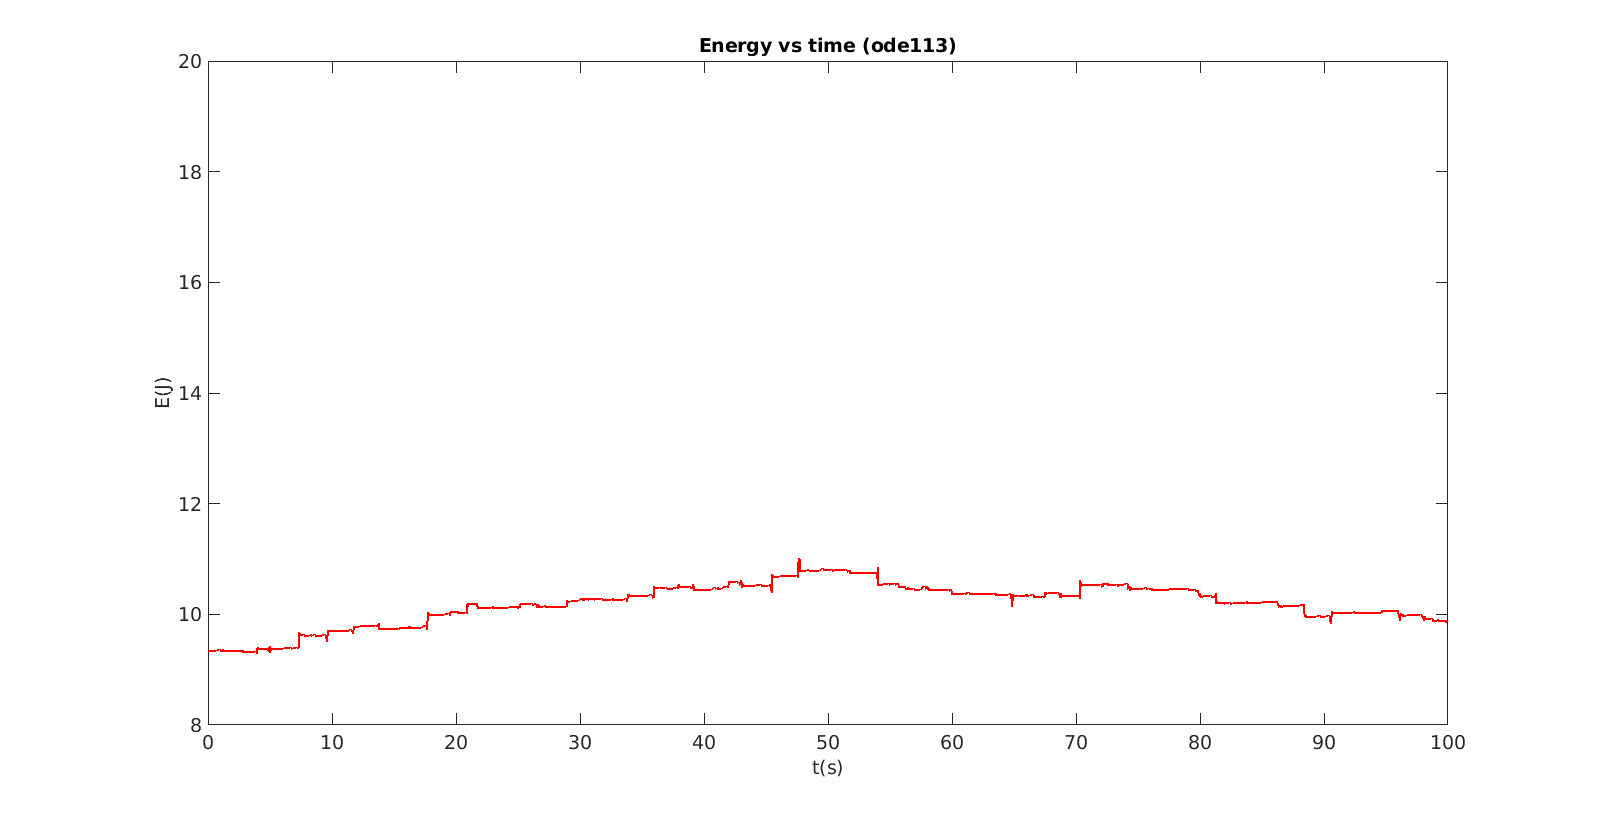
\includegraphics[width=\textwidth]{e_time_ode1113_bigAng.png}
    \label{fig:f1}
  \end{subfigure}
  \hfill
  \begin{subfigure}[b]{0.5\textwidth}
    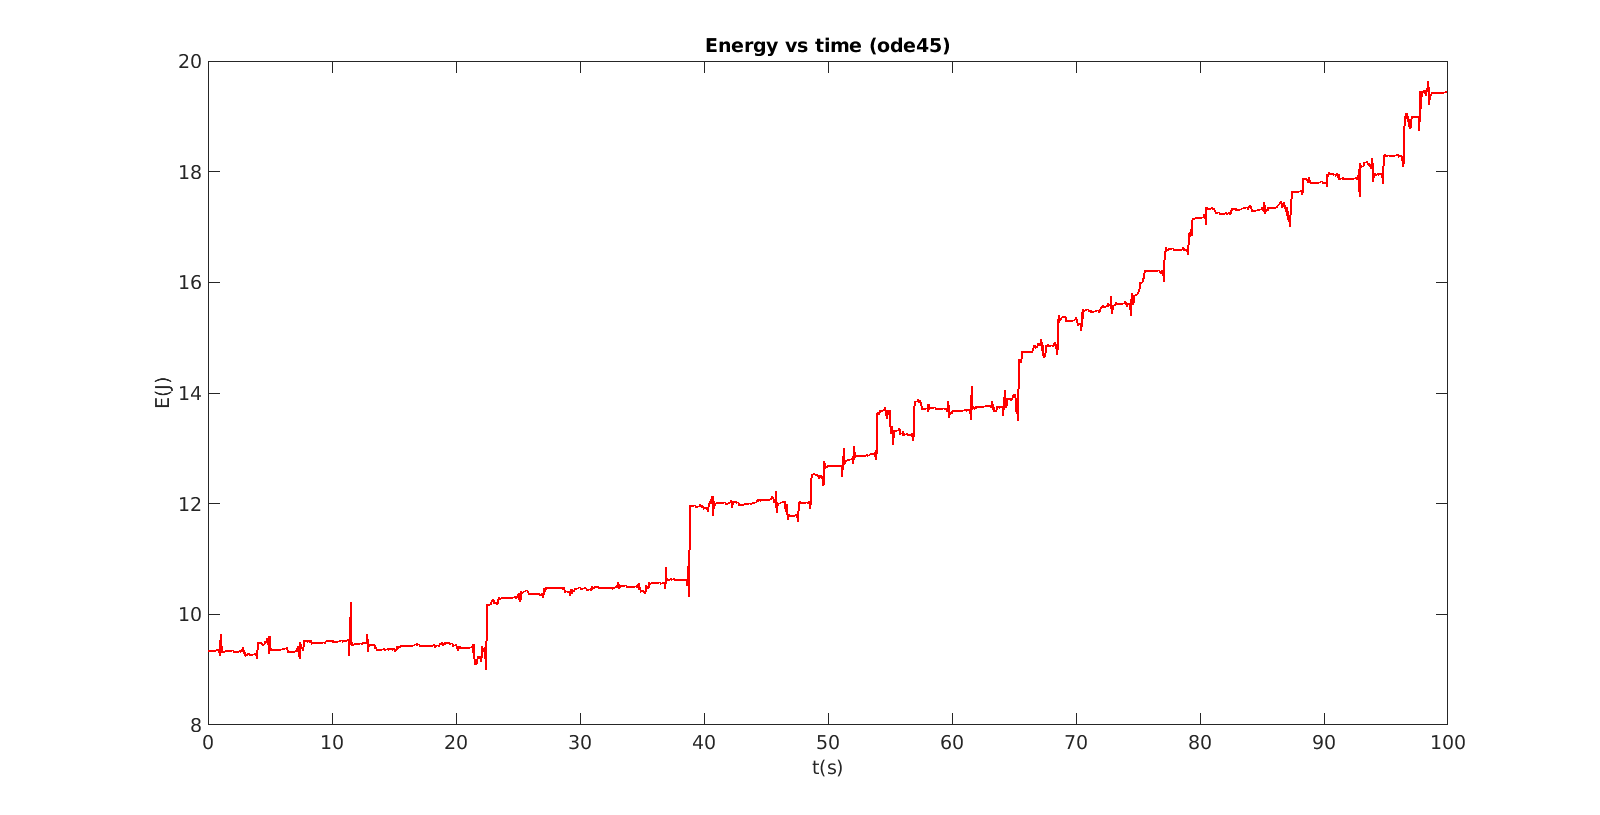
\includegraphics[width=\textwidth]{e_time_ode45_bigAng.png}
    \label{fig:f2}
  \end{subfigure}
  \caption{Total energy plotted against time of the double pendulum using ode113 on the left and ode45 on the right}
\end{figure}

As we can see, ode113 gives a much better error rates. Hence, ode113 is used for the rest of the article.



% insert ode

\section{Dynamics of Double Pendulum and Chaos}

To see the difference in trajectories between two different initial conditions, $\theta_1$, $\theta_2$ are plotted against time $t$.

\begin{figure}[!htbp]
  \begin{subfigure}[b]{0.5\textwidth}
    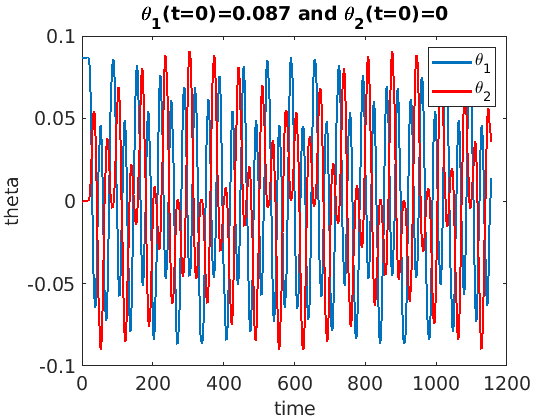
\includegraphics[width=\textwidth]{smallAngle.png}
    \caption{Small-angle release}
    \label{fig:f1}
  \end{subfigure}
  \hfill
  \begin{subfigure}[b]{0.5\textwidth}
    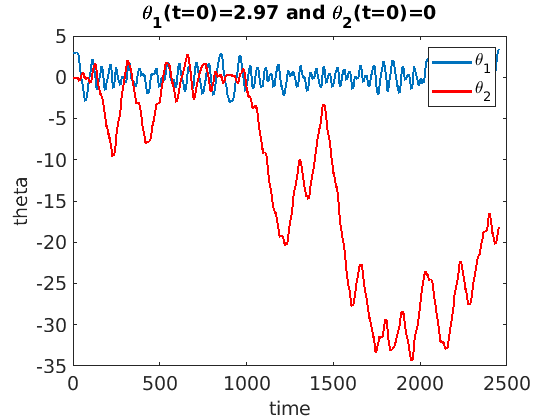
\includegraphics[width=\textwidth]{largeAngle.png}
    \caption{Large-angle release}
    \label{fig:f2}
  \end{subfigure}
  \caption{Angular displacement of $\theta_1$ and $\theta_2$ versus time of small-angle and large-angle release}
\end{figure}

To explain the staggering difference between the two cases above, note that in the case of small-angle release, the trigometric terms sine and cosine of $\theta$ can be approximated as $\theta$, which eliminates the nonlinearity of the equations. The above figure on the left confirms this as the motions of the two bobs are fairly periodic.

In the right figure, two bobs' motions are no longer periodic, with the second bob's angle swings back and forth over a long range, in contrary to the first bob.

Let's see what the graphs of displacement will look like if we modify the initial displacement of $\theta_1$ a bit: $\Delta \theta_{0,1} = 0.001$ over 2500 timesteps, with three cases: $\theta_1(t=0)=2.966$, $\theta_1(t=0)=2.967$ and $\theta_1(t=0)=2.968$.

\begin{figure}[!htbp]
  \begin{subfigure}[b]{0.5\textwidth}
    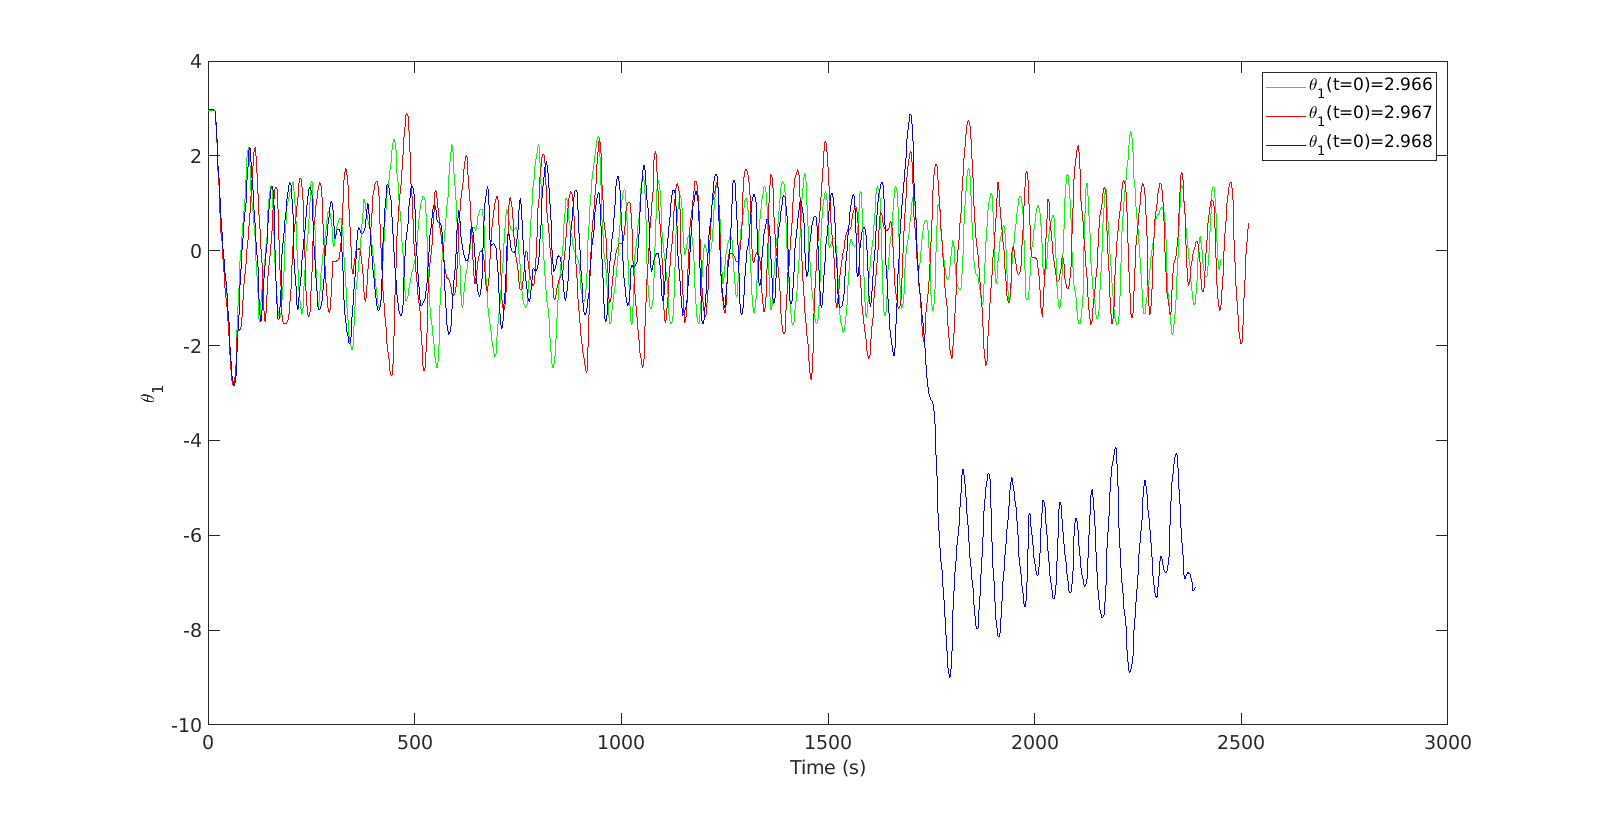
\includegraphics[width=\textwidth]{theta1.png}
    \caption{$\theta_1$ trajectory}
    \label{fig:f1}
  \end{subfigure}
  \hfill
  \begin{subfigure}[b]{0.5\textwidth}
    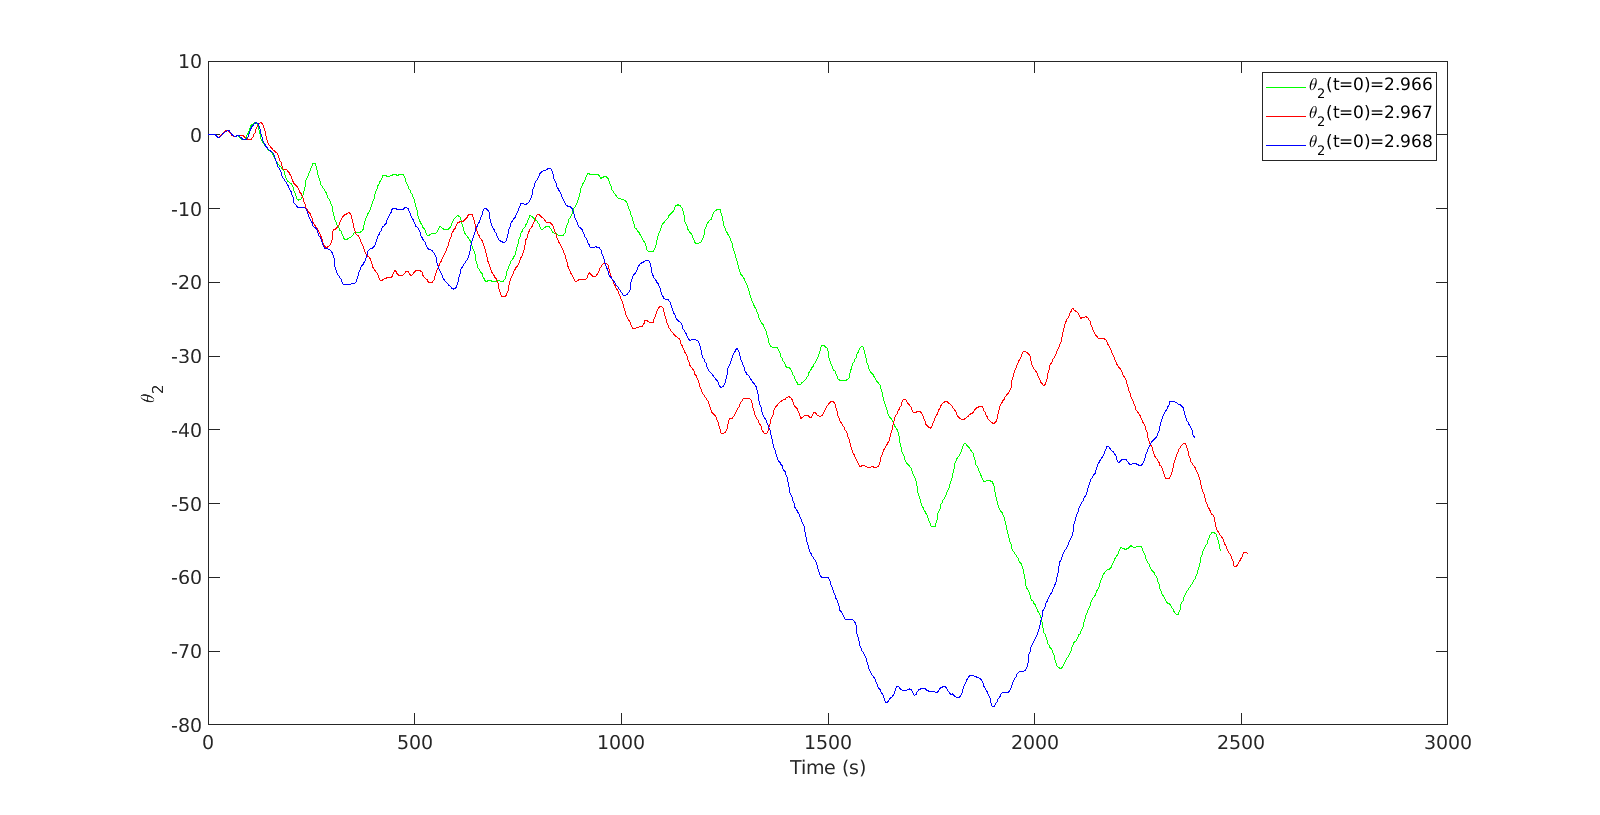
\includegraphics[width=\textwidth]{theta2.png}
    \caption{$\theta_2$ trajectory}
    \label{fig:f2}
  \end{subfigure}
  \caption{Trajectories of $\theta_1$ and $\theta_2$ with different initial displacement of $\theta_1$: $\theta_1(t=0)=2.966$, $\theta_1(t=0)=2.967$ and $\theta_1(t=0)=2.968$}
\end{figure}

On the left hand side, for the first 1800 timesteps, the trajectories of $\theta_1$ are fairly similar and periodic. However after $t > 1800$, $\theta_1$ for the blue line starts to level off, while the other two are still somewhat periodic. In contrast, the movements of the the second bob are nonperiodic from the beginning, and the three lines rarely resemble the other ones. 

The quasi-periodicity of the first bob can be further seen in the ensuing plots of the positions of bob 1 and 2 over time. For illustrative purposes, only plots of $\theta_{0,1} = 2.966$ and $\theta_{0,1} = 2.968$ over the span of 100s are shown. Clearly, the system of double pendulum is extremely sensitive to initial conditions. 

\begin{figure}[!htbp]
  \begin{subfigure}[b]{0.5\textwidth}
    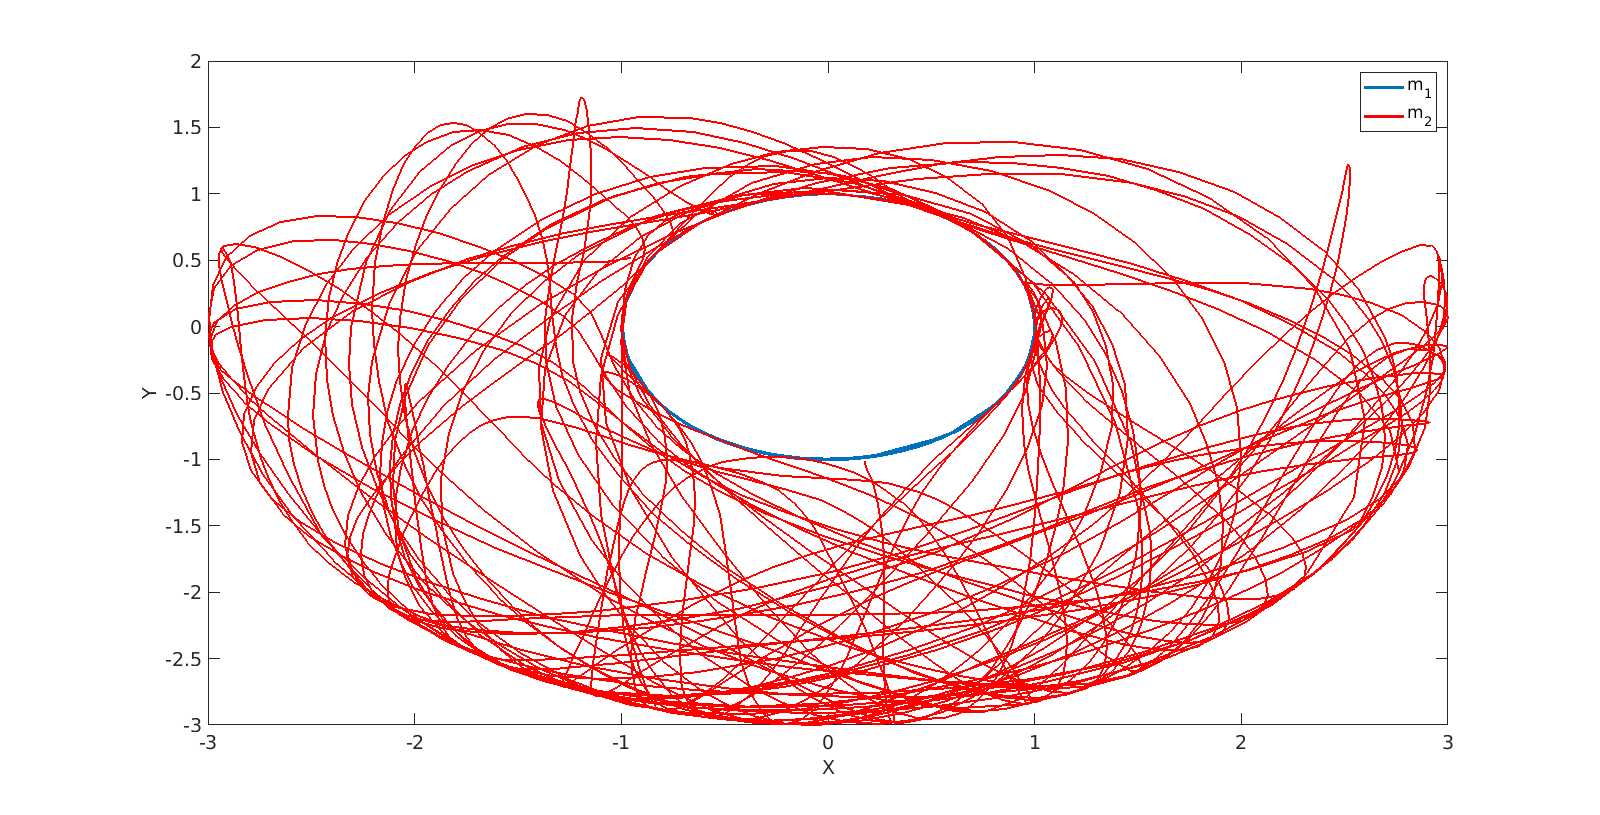
\includegraphics[width=\textwidth]{bob66.png}
    \caption{$\theta_{0,1} = 2.966$.}
    \label{fig:f1}
  \end{subfigure}
  \hfill
  \begin{subfigure}[b]{0.5\textwidth}
    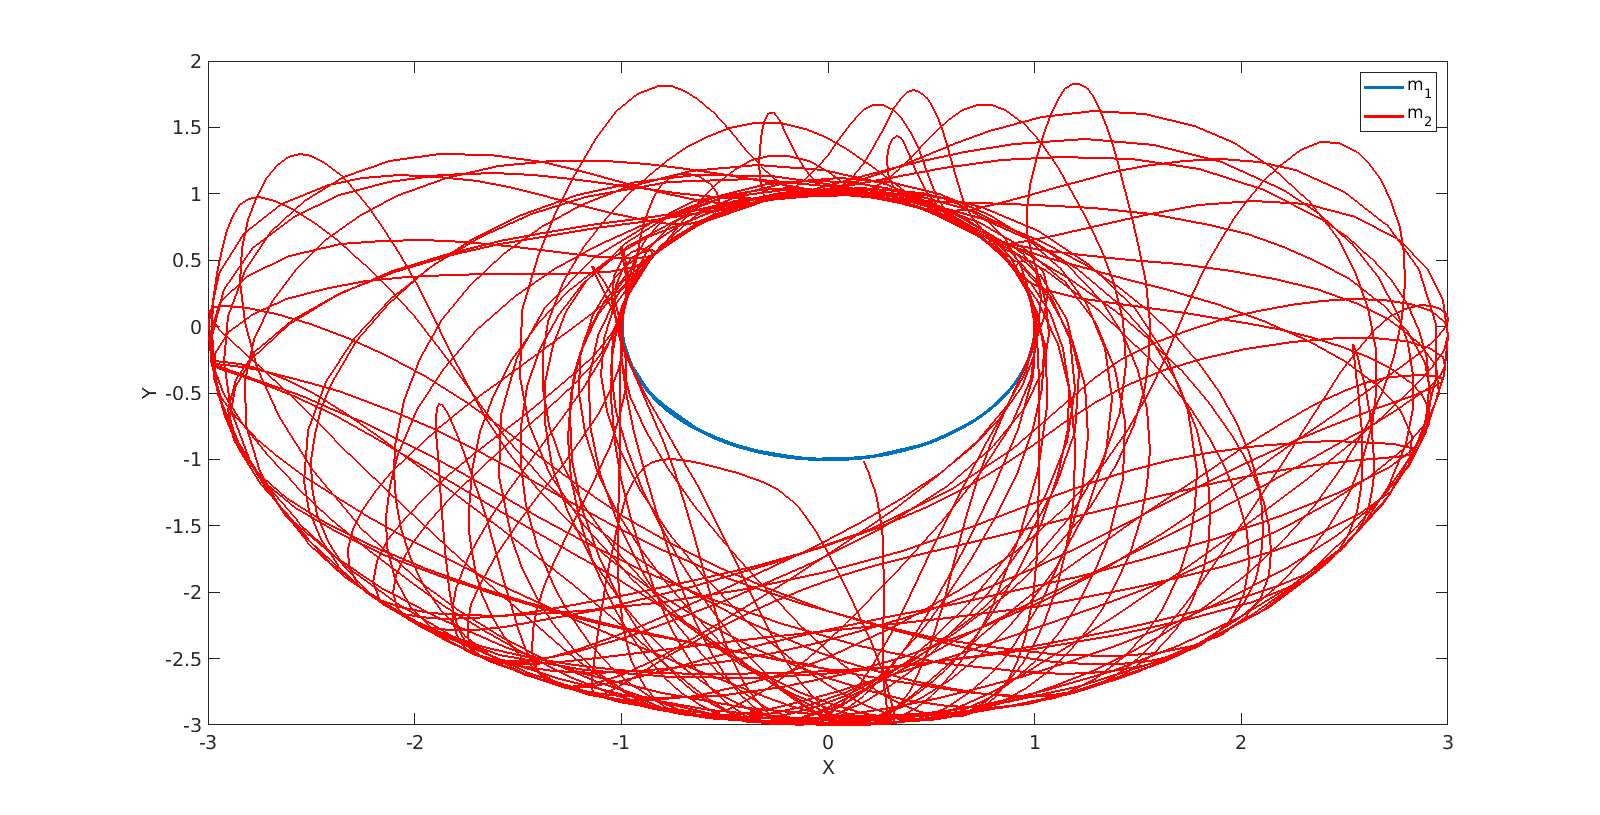
\includegraphics[width=\textwidth]{bob68.png}
    \caption{$\theta_{0,1} = 2.968$.}
    \label{fig:f2}
  \end{subfigure}
  \caption{Positions of bob 1 and bob 2 over time with differential initial displacements.}
\end{figure}


Here, nondimensionalization shines as it predicted the periodicty of bob 1 with $\omega^2 = g/l_1$.

% rewrite the rest of the document, start from here
Be that as it may, we need to find a way to quantifying what makes a dynamical \textit{chaotic}. In numerical methods, one often encounter the spectrum of Lyapunov exponents as a way to characterize chaos. Typically, the dynamical system will have as many Lyapunov exponents as the number of variables in the phase space. 


First of all, if we start with two arbitarily close initial conditions separated by $d_0$, the distance after time t between the orbits in phase space, $d(t)$, diverge very quickly after a short period of time. Thus

\begin{equation} \label{1}
d(t) = d_0 e^{\lambda t}
\end{equation}

where $\lambda$ is the Lyapunov exponent.

Since there are four Lyapunov exponents, we will try to average the Lyapunov exponent to see the general direction of divergence of the system. The average Lyapunov exponent can be taken as the average of $nth$ successive Lyapunov exponents. From 
\begin{equation}
d(t) = d_0 e^{\lambda_i (t_i - t_{i-1})}
\end{equation}

where $i = 1, \ldots, n$ and with some manipulation we have

\begin{equation}
\lambda_i = \frac{1}{t_i - t_{i-1}}ln(\frac{d(t_i)}{d_0})
\end{equation}

but $t_1 - t_0 = \ldots = t_n - t_{n-1} = \Delta t$, find the sum of all those values divided by n, and let $\tau = n\Delta t$, we obtain

\begin{equation} \label{eq 5}
\begin{split}
\lambda &= \frac{\lambda_1 + \lambda_2 + \ldots + \lambda_n}{n} \\
		&= \frac{1}{\tau}\sum_{i=1}^{n}ln(\frac{d(t_i)}{d_0})
\end{split}
\end{equation}

We can see that the unit of $\lambda$ is inverse time: $s^{-1}$. 

Let's examine the Lyapunov exponents in details. If the series of $\{x_1, x_2, \ldots\}$ is periodic, that is, the trajectory eventually repeats itself, then $d(t)$ would be approaching close to zero, making $\lambda \rightarrow 0$ as well. Thus, the orbit is neither converging or diverging. For the case of $\lambda < 0$, the orbit is converging toward a sink. Finally, when $\lambda > 0$, the orbit is diverging. The latter is the prime indicator of chaos. Visualization of behavior of $\lambda$ can be found on the figure on the next page.

\begin{figure}[!htbp]
    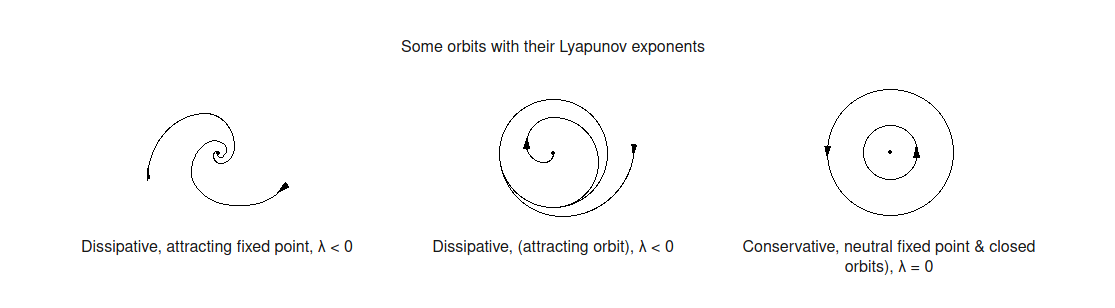
\includegraphics[width=\textwidth]{orbit.png}
  \caption{Three cases of orbits with their Lyapunov exponents}
\end{figure}


Details of numerical methods for calculating the Lyapunov exponent can be found at Sprott. The following calculation of Lyapunov exponent for a similar system to the one in this article is performed by Chen: When the initial angular displacement system is small, $\lambda = 0.0378 s^{-1}$, corresponding to the periodic behavior of the system. On the other hand, in the case of large-angle release, $\lambda =  1.7421 s^{-1}$, which suggests chaos.

Why "suggests", but not "proves"? Generally, a positive Lyapunov exponent is a necessary but not sufficient for chaos. A counterexample can be found in the Perron effect of largest Lyapunov exponent of sign inversion.

\section{Stability of fixed points}

To investigate the stability of the fixed points of the system, we need to find the constant solutions to (31), (32), (33), and (34), of the form $\{\theta_1, \theta_2, \dot\theta_1, \dot\theta_2\}$. Setting the left hand sides of all those equations to 0, we get

\begin{equation}
\begin{split}
v_1 = 0 \\
v_2 = 0 \\
M\sin\theta_2\cos(\theta_1 - \theta_2) - \sin\theta_1 = 0 \\
\sin\theta_1\cos(\theta_1 - \theta_2) - \sin\theta_2 = 0
\end{split}
\end{equation}

From which the solutions of $\{\theta_1, \theta_2\} \in \{k\pi \,|\, k \in \mathbb{Z}\}$. The four equilibria of the system are then

\begin{itemize}
	\item $\{0, 0, 0, 0\}$
	\item $\{\pi, \pi, 0, 0\}$
	\item $\{\pi, 0, 0, 0\}$
	\item $\{0, \pi, 0, 0\}$
\end{itemize}

Our next step is to linearize the system of differential equations at equilibria. Define $\bm{\theta} = \left[\begin{smallmatrix}\theta_1 \\ \theta_2 \\ \dot\theta_1 \\ \dot\theta_2\end{smallmatrix}\right]$, we can rewrite the our dynamical system as
\begin{equation}
\frac{d\bm{\theta}}{dt} = J\bm{\theta}
\end{equation}

Where $J$ is the 4-by-4 Jacobian matrix of partial derivatives of $\bm{\theta}$ with respect to its four coordinates. Substituting the equilibrium points into the Jacobian matrix to find eigenvalues will give insight into the behavior of those points. Further classification of equilibria is unfortunately out of scope for this article. However, the stability of fixed points can be generally be divided into three cases:

\begin{itemize}
	\item The equilibrium is \textit{asymtotically stable} if the initial guesses starting near the equilibrium tend to it asymptotically as $t\rightarrow 0$
	\item If all initial guesses in a small enough neighborhood of the equilibrium are \textit{attracted} to the it, then the latter is \textit{stable}.
	\item The equilibrium is \textit{unstable} if all initial guesses in a small enough neighborhood of the equilibrium \textit{repel} it.
\end{itemize}

\section{Conclusion}
Nondimensionalization is not the only way to simplify systems of nonlinear equations. It is not mandatory to use nondimensionalization to solve the a nonlinear system numerically. Although the idealized system of double pendulum is deterministic, its longterm behavior is unpredictable as extreme sensitivity to initial conditions perturbs the trajectory exponentially. Careful treatment of the classification of fixed points of the idealized system of double pendulum is expected in the future work.
\newpage
\bibliography{ref}
\bibliographystyle{plain}
\nocite{*}

\end{document}